%% Introduction

\section{Background and Motivation}
\
\
\
\
The world population is growing at an exponential rate, so is the energy requirement. Conventional energy sources like fossil-fuel based generators, nuclear power plants and hydro power plants have served us good so far, but at an environmental and climatic cost. With green house emissions from thermal power plants there has been a considerable climate change. The radioactive cores of the nuclear power plants are highly toxic waste; moreover, the right of way for hydro power stations is becoming more and more difficult owing to the regional ecological damage it causes. In addition the fossil-fuels are being depleted at an alarming rate. Hence, governments and industries all around the world are taking initiatives to replace conventional energy sources with green energy sources like solar and wind; for e.g. India's Solar Policy states for a 100 GW solar generation capacity by end of year 2022.\\

However, there is a fundamental difference between the conventional and renewable energy generation. The renewable energy generation cannot be precisely planned as it is weather dependent. Solar energy generation is dependent on irradiance, temperature, wind speed and cloud cover; whereas wind energy generation is dependent on wind speed, temperature, pressure and humidity. This causes high variability and seasonal deviations in energy generation; moreover, it does not follow the load demand profile. Thus, integration of large amounts of solar and wind generators in the power grids can lead to lowered reliability and stability.\\

In order to increase the penetration of renewable energy generators in the conventional power grid, forecasts at multiple time horizons can play an important role; as good forecasts can make possible effective planning of renewable energy generation. Also, highly accurate forecasts can help in grid regulation, power scheduling, unit commitment and load-following. In short, a good forecast can help us model renewable energy generation as in the conventional sense, making the system operators work easy. Therefore, the study of different forecasting methodologies for solar and wind energy generation is a seminal step in developing a power grid which has renewable generation as its largest component.\\

Moreover, with the aim to gain energy independence and reduce the carbon foot-print India is actively pursuing an unprecedented expansion of its renewable energy sector (especially Solar and Wind energy sector). The Indian goal for massive expansion of its renewable energy sector will be a paradigm shift in its otherwise conventional energy dependent energy infrastructure.
As of 31st November, 2015 India has a total of 275.9GW of electrical energy capacity installed of which only 76.57GW (27.75\%).(Electricity sector in India, n.d.) comes from renewable resources (includes all, Biomass, Small Hydro, Waste to Power, Wind and Solar). Wind Energy accounts for 24.76GW (8.9\%) and Solar Photovoltaic (SPV) accounts for 4.68GW (1.69\%) (Renewable energy in India, n.d.).\\

India has set target of year 2022 when it will have an additional 100GW from SPV and an additional 60GW from Wind Farms (Blog: Big Data Improves Renewable Power Forecasts. Will It Help India?, 2015)Hypothetically, if every other conventional energy source and renewable energy sources (except Solar and Wind) remains constant till 2022, then we will have a total installed capacity of 435.9GW (58\% increase in installed capacity in 7 years), SPV and Wind together will contribute about 189.44GW (43.5\%). That is a tremendous increase in the renewable energy installed capacity.

\begin{figure}[H]
\centering
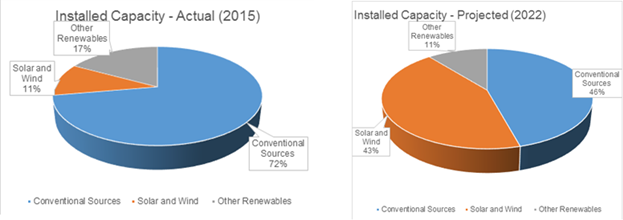
\includegraphics[scale=1]{Intro1}
\caption{Actual and Projected Installed Electricity Generation Capacity Distribution}
\label{figc1h1} %% to refer use, \ref{}
\end{figure}

The Indian electricity grid is working in an archaic mode, where it’s operational practices and control mechanisms are tuned to serve a grid dominated by Thermal Power Stations (Fossil Fueled and Nuclear) which provide for base load and Hydro Power Stations providing for peak load. The energy output of these two kinds of power plants is deterministic and hence are easier to schedule.\\

But, the energy output of Solar and Wind Power Plants depends on the weather conditions and is stochastic and not deterministic and on most occasions delivers power lower than its installed capacity, which is a real problem for grid operators. Only an accurate forecast of power can solve the problem of efficient renewable energy scheduling (Electricity sector in India, n.d.).\\

At the moment there have only been two pilot projects for wind energy forecasting; one in Gujarat that completed in February 2015 with 30\% inaccuracy of forecasts; not due to the inefficiency of the participating companies (all were foreign private companies) but due to the lack of data; the other one has started in Tamil Nadu by a company called Vortex in cooperation with NIWE (National Institute of Wind Energy). There is no forecasting pilot project for solar yet ( Richts, Strauß, & Heinemann, 2015).\\

Hence development of an indigenous renewable energy/power forecasting application for solar photovoltaic and wind power plants is of paramount importance. So that, by 2022 when almost 43\% of the installed generation capacity will consist of SPV and Wind power plants, we will have a robust renewable generation forecasting application to take care of the intermittent nature of energy generation.




\section{Literature Review}
\
\
\
\
Owing to the stochastic nature of the weather variables (Irradiance, Temperature and Wind Speed), the energy/power generation output from Solar Photovoltaic (SPVPP) and Wind Turbine Power Plants (WTPP) is also stochastic i.e. undeterministic. The control and operation of conventional electricity grids depend on the assumption that generation is deterministic and the load is undeterministic. Hence, it becomes a great challenge to perform optimal scheduling, unit commitment and load-balancing in grids where there is a large penetration of SPVPs and WTPPs without accurate generation forecasts.
It is self-evident that that undeterministic generation from SPVPs and WTPPs is the direct result of the stochastic nature of the weather variables which drive these systems. Therefore, for accurate generation forecasting of these systems, we need to forecast the driving weather variables accurately. These forecasted weather variables can then be fed as inputs to the deterministic energy/power estimation models for SPVP and WTPP as described in (Masters, 2004) and (Patel, 2006) respectively. Hence, the forecasting should done for driving weather variables, and the energy/power forecasts for SPVPs and WTPPs should be done indirectly by using the energy/power estimation models. 
A holistic study of the current techniques used for weather variable forecasting shows us that Autoregressive Integrated Moving Average models (ARIMA), Artificial Neural Networks (ANN) and Numerical Weather Prediction systems (NWP) are at the forefront of the forecasting technology horizon. ARIMA and ANN are accurate for intra-hour and intra-day irradiance forecasting; whereas NWPs like ECMWF (European Centre for Mesoscale Weather Forecasting) and WRF (Weather Research and Forecasting) are accurate for day-ahead irradiance forecasting ( Diagna, David, Lauret, Boland, & Schmutz, 2013). ANN with back propagation can be used successfully for wind speed forecasts, and similar ANN models can be used for forecasting other weather variables like Dew-Point Temperature, Relative Humidity, Wind Direction and Pressure (Upadhyay, Choudhary, & Tripathi, 2011). ANN and ARIMA are good for short-term wind speed forecasting, whereas NWP models predict wind speed better than statistical models; moreover, hybrid models employing combination of the before mentioned techniques are the most accurate for wind speed prediction ARIMA (Saroha & Aggarwal, 2015).  ANN and NWP are the best model choices for wind speed prediction ( Zhu & Genton, 2012). Hence, we can conclude that ARIMA, ANN and NWP methods are a good choice for short-term (intra-hour and intra-day; ANN and ARIMA) and long-term (day-ahead; NWP) weather variable forecasting; in addition, hybrid forecasting models based on these techniques can improve the accuracy of the forecast (Chang, 2014).\\

The classical method of time series modelling propagated by the statisticians Box and Jenkins in the 70’s, and still used today. Their models of ARMA (Autoregressive Moving Averages, for stationary time series) and ARIMA (Autoregressive Integrated Moving Averages, for non-stationary time series) provide building blocks for creating the most basic statistical forecasts based on the time series’ mean and variance values. ARIMA models for weather forecasting are developed by examining Auto-Correlation Function (ACF) and Partial Auto-Correlation Function (PACF), the best models are selected based on the lowest values of Akalike Information Criterion (AIC) and Bayesian Information Criterion (BIC) ( Shamsnia, Shahidi, Liaghat, Sarraf, & Vahdat, 2011). Hybrid models consisting of Multi-Linear Regression (MLR) and ARIMA outperform usual ARIMA and ANN models for weather prediction (Sharma, 2012). ARIMA and Artificial Neuro Fuzzy Inference System (ANFIS) are compared for weather forecasting, it is observed that AFIS performs better than ARIMA, as it is a hybrid system (Tektas, 2010). ARIMA and ANN both are good for time series weather forecasting, however hybrid ARIMA-ANN outperforms both techniques by reducing model uncertainty (Zhang, 2003). For short-term irradiance forecasting ARIMA models outperform NWP, and predict accurately in the time frame of 5 minutes to 4 hours, but NWP perform superiorly better for day-ahead irradiance forecasting ( Prajapati & Sahay, 2016) and ( Kaushik & Singh, 2008).ARIMA models have been developed using Box-Jenkins methodology for predicting accurately monthly values for temperature, rainfall and relative humidity in Ahvaz, Iran and districts of Sri Lanka (Sarraf, Vahdat, & Behbahaninia, 2011), (Partheepan & Jeyakumar, 2005) and (Nurry, Koch, & Alam). Non-Linear Autoregressive Exogenous Artificial Neural Network (NARX) performs better than ARIMA being a non-linear model for wind speed time series one-step ahead prediction (Cadenas, Rivera, Campos-Amezcua, & Heard, 2016). Hence, ARIMA models have been applied successfully for short-term forecasting of irradiance, temperature and wind speed, using the ACF and PACF examination approach in combination with AIC and BIC for selecting the best model; moreover, hybrid models of ARIMA with other techniques are superior but complex as compared to usual ARIMA models for weather variable prediction.\\

The modern technique of Artificial Neural Networks, which are inspired from biological neural networks. They work on the principle of interconnected neurons forming a network between inputs and outputs; the neurons consists of a mathematical function, biases and weights. This network of neurons is made to learn the data during training phase using appropriate learning methods. ANN’s can be trained to do a variety of jobs; namely Clustering, Classification and Regression. For weather variable forecasting we need to develop a neural network for solving a regression problem. ANN trained with back propagation (BP) algorithm can approximate large class of non-linear functions; hence, it can be used in weather prediction, the only requirement for good predictions being good quality historical data (Reddy, Devi, Kumar, Reddy, & Nayak, 2012).  Multi-Layer Perceptron model (MLP) has the potential to be successfully applied to weather forecasting (Kumar & Jha, 2013). MLP with BP is an ideal solution for predicting dynamic and non-linear weather processes, it is better than traditional numerical methods (Malik, Singh, & Arora, 2014). Various weather variables like rainfall, wind speed, irradiance and temperature can be forecasted accurately using MLP and Radial Basis Function Network (RBFN) (Shrivastava, Karmakar, Korwar, & Guhathakurta, 2012). . When MLP RBFN, Elman Recurrent Neural Network (ERNN) and Hopfield Model (HFM) are compared, MLP and RBFN perform weather accurate weather forecasts comparatively (Maqsood, Khan, & Abraham, 2004). A hybrid model using ARIMA which is a linear model and ANN which is a non-linear model, irradiance can be predicted accurately for both clear and cloudy days ( Voyant, Muselli, Paoli, & Nivet). To improve irradiance forecasts further additional inputs of irradiance derivatives can be used, which improves irradiance forecast under changeable weather conditions (Wang, et al., 2016). For a shot-term irradiance forecast ANN outperforms NWP (Cornaro, et al.). Also, temperature prediction with greater accuracy can be done by training one ANN model for each season (Hayati & Mohebi, Temperayure Forecasting Based on Neural Network Approach, 2007). Ensemble ANN model for temperature forecasting improves accuracy to a great extent (Kadu, Wagh, & Chatur). ANN outperforms ARIMA model for short-term wind speed forecasting (Catalao, Pousinho, & Mendes, 2009). Hence, incorporating ensemble and hybrid modeling strategy with ANN can help predict irradiance, temperature and wind speed to a high accuracy for a short-term forecast.\\

The Numerical Weather Prediction Models (NWP’s) like ECMWF and WRF they produce good weather forecasts up to 1km spatial and about 3min temporal resolution. NWP’s are quite different from the first two forecasting techniques as they depend on accurate physical descriptions of the atmospheric processes and tend to give highly accurate forecasts. But, the problem here is these softwares require supercomputers to run them as they require a lot of computing power and memory. The WRF is a next generation NWP with efficiency, portability, maintainability and extensibility at its core architecture; being open source and community driven, it has fostered communication, cooperation, collaboration within WRF working groups specializing in regional climate, air quality simulation, and NWP research (MICHALAKES,, et al., 2005). WRF model was used for forecasting energy production of a SPVP, WRF weather variables and the historical plant power production data was used to train a Quantile Regression Forest forecast model; it is observed that accuracy of daily energy forecasts is greater than hourly predictions (Almeidaa, Lamigueirob, & Narvarte). Improved power forecast for SPVP and WTPP is carried out using a hybrid model of linear regression of forecasted outputs of the WRF model, this model outperforms the usual WRF model ( Avolio, et al., 2016).  The GHI prediction from WRF are not accurate, but are usually over-estimated due to WRF’s inability to model clouds, aerosols, ozone properly also the radiation models used in WRF are good drivers for atmospheric processes but not so much for precise surface solar irradiances; hence post processing of GHI is required for accurate prediction, some methods are: Spatial Averaging, Incorporating Ozone and Aerosols using satellite retrievals, Kalman Filters, and Recursive method and Assimilating cloud cover data into the WRF initialization using GOES satellite imagery; as mentioned in (Larson, Nonnenmacher, & Coimbra, 2016), ( Lara-Fanego, Ruiz-Arias, Pozo-Va´zquez, Santos-Alamillos, & Tovar-Pescador, 2011), (Rincón, Jorba, Baldasano, & Monache, 2011), (Mathiesen, et al., 2014) and (Heinemann, Lorenz, & Girodo) respectively. Another method to improve the GHI forecasts from the WRF, an ensemble WRF model is suggested where linear combination of one or more WRF runs for the same location with different initial and boundary conditions is done, this improves the GHI forecast by reducing the uncertainty associated to the initial and boundary meteorological conditions (Díaz, Souto, Rodríguez, Saavedra, & Casares, 2012). The land surface schemes responsible for computing heat and moisture fluxes over the land surface overestimate, for improving the temperature and wind speed forecast from WRF model a good post-processing system has to be used ( Khvorostyanov, Menut, Dupont, Morille,, & Haeffelin). The YSU scheme in WRF with an ensemble mean with a GFS (Global Forecast System) initialized WRF model is the best for wind speed prediction ( Rabideau). The ARW user manual provides excellent documentation of the installation and running of the WRF software (Wang, et al., 2016). The comparison of the two dynamic solvers within WRF which are the Advanced Research WRF (ARW) and the Non-hydrostatic Mesoscale Model (NMM), shows that there is no difference in the WRF output with the change in the dynamic solvers ( Bernardet, et al.). Hence, WRF is proved to be a great tool for mesoscale weather prediction and it has been used successfully for day-ahead weather forecasting in relation to SPVP and WTPP generation forecasting; moreover, with good parameterization of the WRF model options, appropriate post-processing systems and ensemble models the WRF system can be used for very accurate day-ahead forecast of the SPVP and WTPP generation.\\

To summarize, the problem of solar and wind energy/power forecasting can be broken down into two parts: the energy estimation part and the weather variable forecasting part. The weather variable forecasting can be done using ANN and ARIMA for short-term i.e. intra-hour and intra-day periods; whereas NWP like WRF can be used for day-ahead forecasting of weather variables. These forecasted weather variables can then be used as input to the energy estimation models which will compute the forecasted energy/power for the SPVP and WTPP. A HADOOP based ARIMA weather forecasting has been developed using HBASE and SQOOP for database management, this shows that for forecasting systems to be scalable and usable they have to be developed as an application so that routines are automised (Li, Ma, Liu, & Fan, 2013). Figure 3 shows the schematic of the forecasting procedure, but in order to achieve this an indigenous application has to be designed and developed; which will make it easy to train and develop ANN and ARIMA models as well as automate the process of running a WRF, and energy estimation of SPVP and WTPP. This thesis intends to develop a complete application which can function as a platform for solar and wind energy estimation and forecasting.


\section{Contribution to Scientific Community}
\
\
\
\
The process of generation forecasting of SPVP and WTPP includes: Data acquisition, Data pre-processing, Selection of appropriate mathematical forecasting model (i.e. ARIMA, ANN or WRF), Forecast model development, Forecast model testing and finally the Forecast model implementation. All these steps require different softwares and/or Application Programming Interfaces (API's) to work as a cohesive unit to get forecasting done. The work done in this thesis tries to bring together all the aforementioned steps under one umbrella, to make the forecaster's job a little lucid. The Fig (\ref{figc1h2}) shows the block diagram of forecasting model developed, here the stochastic weather variables are forecasted using the different mathematical models, and these forecasted weather variables are fed as inputs to the deterministic energy estimation models for SVPP and/or WTPP to get the energy/power forecasts as desired.
`	`																		`  

\begin{figure}[H]
\centering
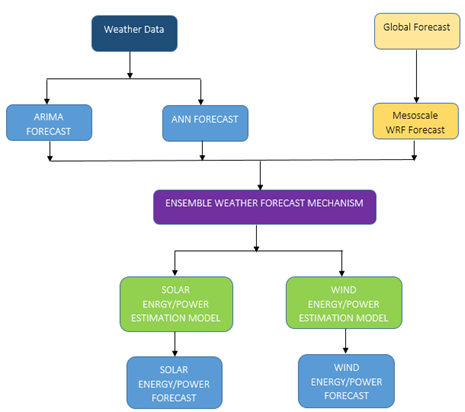
\includegraphics[scale=1]{Intro2}
\caption{Block Diagram – Ensemble Solar/Wind Power Forecasting}
\label{figc1h2} %% to refer use, \ref{}
\end{figure}

The Fig (\ref{figc1h3}) illustrates the application structure developed in MATLAB using its GUI feature. The application performs all the steps mentioned earlier to get the generation forecast through an easy to use GUI interface. Moreover, the application has been coded with modularity at the heart of its design; which makes it easy to upgrade, change and debug as desired by the forecaster. 

\begin{figure}[H]
\centering
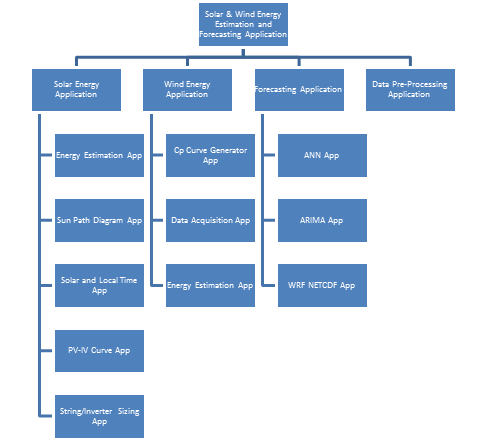
\includegraphics[scale=1]{Intro3}
\caption{Organization Structure of Application}
\label{figc1h3} %% to refer use, \ref{}
\end{figure}

The application can act as a complete software package for energy estimation and generation forecasting for SVPP and WTPP, and be a solid foundation for developing a real-time generation forecasting system.\\